\documentclass[a4paper,12pt]{article}
\usepackage{geometry}
\usepackage{graphicx}
\usepackage{sidecap}
\usepackage{epstopdf}
\usepackage{amssymb}
\usepackage[font={small}]{caption}

%\DeclareGraphicsRule{.tif}{png}{.png}{`convert #1 `dirname #1`/`basename #1 .tif`.png}
\begin{document}


\section*{Intro}
Elucidation of the structural properties of biomolecules is important for many reasons, e.g drug design. Over the years scientists have been able to chemically induce the crystallization of proteins for instance, which when exposed to X-rays yield very bright scattering signals related to the crystalline structure. The technique of protein crystallography analysis has been refined to the point that a simple computer can read in images and return electron densities with the click of a button. Unfortunately, crystal formation itself is an arduous task and is not always readily feasible.
\\*
\\*
We aim to achieve substantial structural information in the absence of an ordered system. Instead of a crystal, which consists of N particles at a single orientation relative to the X-ray beam, our samples consist of N particles, each having an independent orientation. In the absence of inter-particle scattering ( dilute samples and high scattering angles), the infinite photon-limit intensity at time $t$ from such an arrangement is given by 

\begin{equation}
I_{t}( \vec{q} ) = \frac{N}{8\pi^{2}}\int S( \vec{q},\omega ) \, d \omega + \int \alpha_{t}( \omega ) S( \vec{q},\omega ) , d \omega   
\end{equation} 

\noindent where $\omega$ represents the particle orientation in 3-dimensional space, $\alpha_{t}$ is the fluctuation in the number of particles at orientation $\omega$, and 
\begin{equation}
S(\vec{q},\omega) = | \int \rho (\hat{R}(\omega)\cdot \vec{r} ) e^ { -2\pi \vec{q} \cdot \vec{r} } d\vec{r} | ^{2}
\end{equation}

\noindent is the Fourier transform of the electronic density $\rho(\hat{R}(\omega)\cdot \vec{r} ) $ for a particle at orientation $\omega$ ( $\hat{R}(\omega)$ is a 3-dimensional rotation operator ). Kam showed theoretically that a single particle intensity correlation function can be extracted from such a system by averaging intensity correlations from orientation ensembles of particles at different instances in time:

\begin{eqnarray} \label{KAM}
C( \vec{q}_{1}, \vec{q}_{2} ) &\equiv& \int S( \vec{q}_{1},\omega ) S( \vec{q}_{2},\omega ) \, d \omega \nonumber \\
&=&\langle I_{t}( \vec{q}_{1}) * I_{t}(\vec{q}_{2}) \rangle_{t}  - S(|q_{1}| )S(|q_{2}|)
\end{eqnarray}

where

\begin{equation}
S(|q|) = \frac{N}{8\pi^{2}}  \int S( \vec{q},\omega ) \, d \omega .
\end{equation}

\noindent is the orientationally averaged scattering, a quantity that is easily measured. It is important for the particles to remain fixed during each measurement of $I_{t}( q )$ , i.e. the exposure time should be smaller than the characteristic diffusion time of the system under investigation. As we are working in the finite-photon regime, it is also important that the flux be sufficiently high to ensure two photons scatter from the same particle into separate scattering vectors. Therefore, the experimental conditions must be carefully optimized to simulataneously maximize signal and minimize heating. This technique is referred to as Correlated X-ray Scattering ( CXS ) .
\\*
\\*
In principle, $C( \vec{q}_{1}, \vec{q}_{2})$ contains additional information about the internal structure of the scatterers not attainable from simple x-ray scattering measurements. Wochner et al (2009) claimed that local order within disorder could be extracted for colloidal gels of micron sized polymethylmethacrylate beads based on CXS measurement. Artereli et al gave a critical analysis of CXS measurement and the ability to uncover hidden symmetries from a solution of disordered, identical scatterers. It may be expected that CXS can be used to refine an atomic resolution model of the scatterer, thus improving our knowledge of the molecular structure in cases where suitable crystals are not attainable.
\\*
\\*
\noindent In order to benchmark such an experiment, we have performed CXS on silver nanoparticle ( NP ) solutions at the Stanford Synchrotron Radiation Lightsource ( SSRL ) . NP scattering is very specific, so we know which scattering angles should exhibit strong CXS signal. These measuremnents will serve as a benchmark for experiments involving proteins and other more sensitive materials.  

\section*{System , Setup and Data Aquisition}

Our samples consisted of silver NPs in solution. Each particle was roughly 20 nanometers in size, but we observed some particles that were substantially larger. It was important that the particles remained fixed during each exposure, so the sample was cooled to 100 Kelvin using a nitrogen cryo jet. This opposed any heating due to the X-ray beam. The NPs were suspended in a glycerol-based antifreeze in order to prevent the formation of solvent crystals at the low temperature. By monitoring the intensity at constant scattering angle one can check for sample damage and diffusion (Figure needed ), both attributes that the CXS signal is extremely sensitive to.
\\*
\\*
\noindent To house the solutions we used kapton capillaries with a 500 and 600 micron inner and outer diameter respectively. Kapton scatters into relatively lower angles as does glycerol, hence we did not anticipate corrupting our silver NP signal with a large background. 
\\*
\\*
\noindent The experiment was conducted at the micro-crystallography beamline (12-2) at SSRL. Samples were prepared a day early and stored in a liquid nitrogen bath. Samples were loaded and oriented in the X-ray beam using the Stanford Automated Mounting System (SAM ) , controllable from the experimental hutch. Using a liquid nitrogen-cooled double crystal monochromator we tuned the beam energy to 17 keV. The beam was focused down to about 15x15 $\mu m ^{2}$ using Rh coated Kirkpatrick-Baez mirrors.
\\*
\\*
\noindent Images were taken using a Dectris Pilatus 6M pixel detector. Our goal was to record as many images as possible, each one representing a different ensemble of fixed particle orientations. The sample holder was equipped to automatically rotate the capillary about its longitudinal axis. The capillary was oriented such that its longitudinal axis was perpendicular to the beam (Figure needed) and then it was rotated through a 150 degree angle. The photon counts were read out and reset every 0.7 second and every 0.3 degrees or rotation, giving us 500 shots per 150 degree rotational scan. This was deemed an optimal timing to simultaneously maximize signal and minimize damage and heating. The beam was shining on the capillary for the duration of the scan, hence the center of the capillary was constantly heated. However, this effect was negligible given the path length of the beam through the sample ( 500 $\mu$m ). Between scans we moved the capillary longitudinally, so as to always probe different regions of the sample, and hence different ensembles of particle orientations.

\section*{Expected Results}

\begin{SCfigure}
\centering
	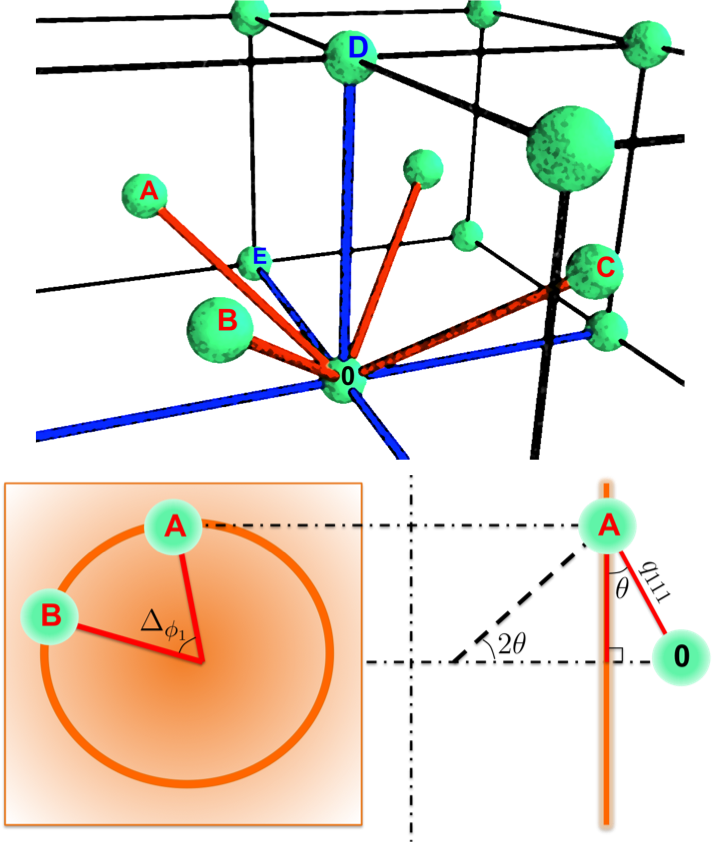
\includegraphics[scale=0.75]{./figure_EXPECTED.png}
	\caption{ \textit{Top} The reciprocal lattice of a \emph{single} silver NP at an aribtrary orientation with 4 of the 8 Bragg reflections (motas) at $q_{111}$ shown in red. Shown in blue are 3 motas at $q_{200}$. Also shown is the point $q=0$ point, labeled by 0. The magnitude of vectors $\vec{A}-\vec{B}$ , $\vec{A}-\vec{C}$, and $\vec{D}-\vec{E}$ are easily calculable using the reciprocal lattice unit cell parameters. For instance, $\left |\vec{A} - \vec{B}\right | = \frac{2}{\sqrt{3}}\,\,q_{111}$. \textit{Bottom} A diagram of the detector and its relation to the reciprocal lattice. The detector probes a plane of reciprocal space. Occasionally, as is shown, two Bragg peaks from the \emph{single} silver NP will intersect this plane, resulting in a positive intensity correlation. }
\label{EXPECTED}
\end{SCfigure}


Each silver NP is a randomly oriented face-centered-cubic lattice, with a corresponding randomly oriented body-centered-cubic reciprocal lattice. As the real space lattice points are atoms, we will refer to the recirpocal lattice points hereafter as motas. In order to measure a double scattering event from a single silver NP, it must be oriented such that at least two motas are simultaneously intersecting the detector. For instance, at constant scattering vector $q_{111}$ there are several orientations which give rise to double scattering events ( Figure ~\ref{EXPECTED} ). The presence of the CXS signal can be determined by performing an auto correlation along the ring of intensities at $q_{111}$:

\begin{equation} \label{COR}
\left \langle I_{t_{i}}( \vec{q}_{111,1}) * I_{t_{i}}(\vec{q}_{111,2}) \right \rangle_{t_{i}} \Rightarrow \left \langle \int_{0}^{2\pi} I_{t} ( q_{111},\phi ) * I_{t} (q_{111},\phi +\Delta_{\phi} )\, d\phi \right \rangle_{t}.
\end{equation}

\noindent Here $\phi$ is the azimuthal coordinate in the plane of the detector, and $\Delta_{\phi}$ is the angle between $\vec{q}_{111,1}$ and $\vec{q}_{111,2}$ when projected onto the detector. Kam theory suggests we should see peaks in this average auto correlation function at $\Delta_{\phi _{1}} = \arccos[ \frac{-2}{3\cos^{2}\theta} + 1  ]$ and $\Delta_{\phi _{2}} = \arccos[ \frac{-4}{3\cos^{2}\theta} + 1  ]$ where $2\theta$ is the standard scattering angle ( Figure ~\ref{BG}). These values can be calculated using elementary geometry.

\section*{Analysis and Results}
\begin{figure}
\centering
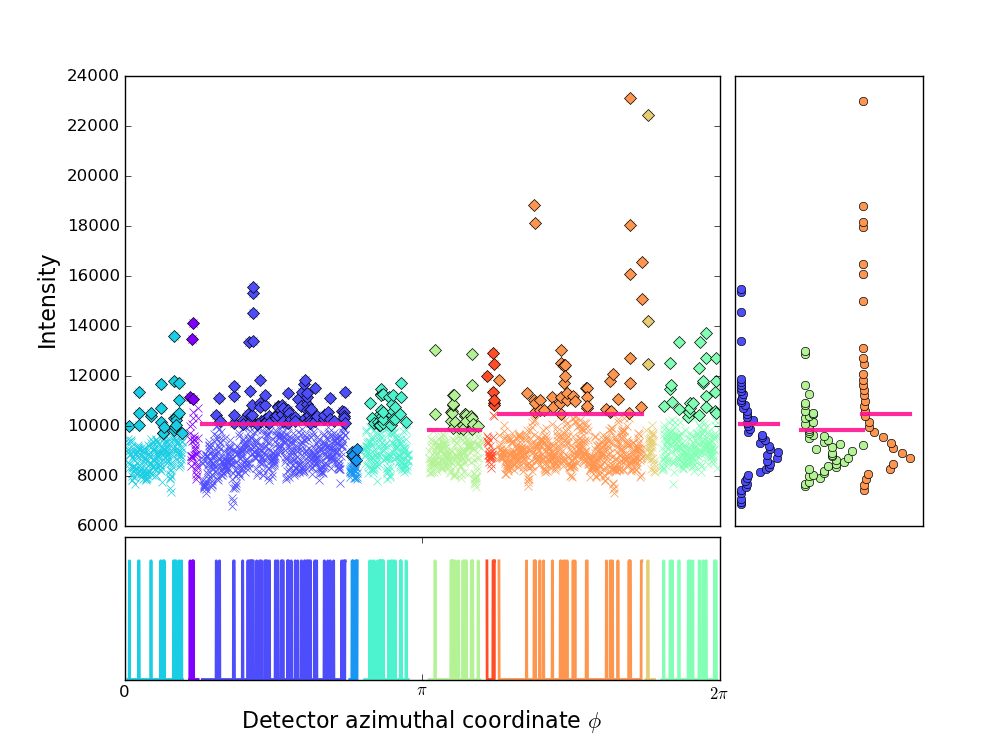
\includegraphics[scale=0.6]{./figure_BINARY.png}
	\caption[font=small]{ Binary filter applied to the intensities around the $q_{111}$ Bragg ring for a single exposure. Each module is treated separately. Different colors correspond to different detector modules, and pink lines denote the binary cutoff, which we set to one standard deviation above the pixel mean of each each module/ring intersection. \emph{Top left} raw interpolated intensities \emph{Top right} Histograms of all intensities at select modules \emph{Bottom} Binary intensities . }
\label{BINARY}
\end{figure}

As each measurement represents a large ensemble of randomly oriented NPs, our detector images display the standard Bragg rings associated with powder diffraction. The detector is made up of 60 electronic modules separated by 1-2 mm gaps, therefore each Bragg ring spans multiple modules depending on the distance from sample to detector and the scattering magnitude of the ring. Each module has 94,965 pixels arranged on a 2-dimensional cartesian grid. We fit a bicubic polynomial to each of these pixel grids and estimated the polar pixel values needed to solve (~\ref{COR}). We carefully located the approximate radius and center of each relevant  Bragg ring with 0.05 pixel unit precision. We had to avoid the gap regions between detector modules when calculating the correlations. The gaps resulted in an information loss of up to 12\% per exposure.
\\*
\\*
\noindent Initial attempts to see convergence of the auto correlation signal at $q_{111}$ were unsuccessful. As shown by Kirian et al and Kam [ref] there is an intrinsic background in the CXS measurement resulting from uncorrelated double scattering events, i.e. scattering events from two particles at different orientations. Furthermore they show that the ratio of correlated to uncorrelated double scattering events is independent of the number of particles in the beam. In addition to the statistical noise, there are several sources of systematic noise present in the experiment. The electronic response of each module seemed to fluctuate for reasons unknown, giving rise to dominant correlations between different detector regions. The polarization properties of the beam and sparse shadows on the detector also contributed to false correlations. Occasionally the beam would pass through a very large particle, which would dominate the intensity around the ring. If this particle happened to be oriented such that 2 of its $q_{111}$ motas were intersecting the detector, then a correlation signal would appear where we expected. However, we are interested in correlations arising from an ensemble of identicle particles, so we regarded these large-particle correlations as noise. All together, these systematic noises were enough to drown our signal which is already fighting against a strong statistical noise.
\\*
\\*
\noindent In order to eliminate any source of systematic noise in the intensity measurement we applied a binary filter to the data: intensities greater than a chosen threshold were set to unity, the rest were set to zero ( Figure ~\ref{BINARY} ). The resulting auto correlations averaged to display peaks as the theory predicted. This confirms that we have indeed measured correlations from a solution of randomly oriented nanoparticles using x-rays produced at a synchrotron.    

\begin{figure}
\centering
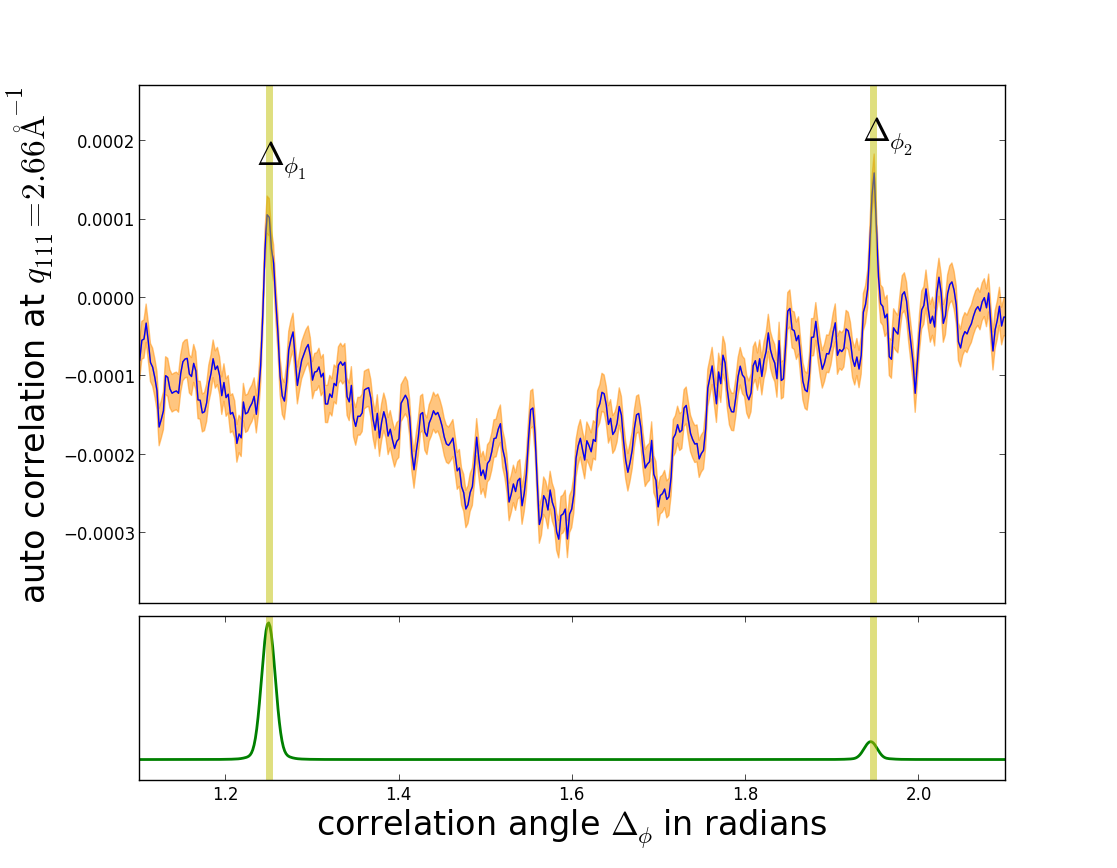
\includegraphics[scale=0.6]{./figure_COR.png}
	\caption[font=small]{ blue is the average of 15k + correlations, orange is the standard error, yellow is the analytical prediction and green is a simulation of 20 nm single particles.}
\label{COR}
\end{figure}

\end{document}